% Options for packages loaded elsewhere
\PassOptionsToPackage{unicode}{hyperref}
\PassOptionsToPackage{hyphens}{url}
\PassOptionsToPackage{dvipsnames,svgnames,x11names}{xcolor}
\PassOptionsToPackage{space}{xeCJK}
\documentclass[
  10pt,
]{article}
\usepackage{xcolor}
\usepackage[margin=0.7in]{geometry}
\usepackage{amsmath,amssymb}
\setcounter{secnumdepth}{-\maxdimen} % remove section numbering
\usepackage{iftex}
\ifPDFTeX
  \usepackage[T1]{fontenc}
  \usepackage[utf8]{inputenc}
  \usepackage{textcomp} % provide euro and other symbols
\else % if luatex or xetex
  \usepackage{unicode-math} % this also loads fontspec
  \defaultfontfeatures{Scale=MatchLowercase}
  \defaultfontfeatures[\rmfamily]{Ligatures=TeX,Scale=1}
\fi
\usepackage{lmodern}
\ifPDFTeX\else
  % xetex/luatex font selection
  \setmainfont[]{Arial}
  \setmonofont[]{Consolas}
  \ifXeTeX
    \usepackage{xeCJK}
    \setCJKmainfont[]{Microsoft YaHei}
  \fi
  \ifLuaTeX
    \usepackage[]{luatexja-fontspec}
    \setmainjfont[]{Microsoft YaHei}
  \fi
\fi
% Use upquote if available, for straight quotes in verbatim environments
\IfFileExists{upquote.sty}{\usepackage{upquote}}{}
\IfFileExists{microtype.sty}{% use microtype if available
  \usepackage[]{microtype}
  \UseMicrotypeSet[protrusion]{basicmath} % disable protrusion for tt fonts
}{}
\makeatletter
\@ifundefined{KOMAClassName}{% if non-KOMA class
  \IfFileExists{parskip.sty}{%
    \usepackage{parskip}
  }{% else
    \setlength{\parindent}{0pt}
    \setlength{\parskip}{6pt plus 2pt minus 1pt}}
}{% if KOMA class
  \KOMAoptions{parskip=half}}
\makeatother
\usepackage{longtable,booktabs,array}
\usepackage{calc} % for calculating minipage widths
% Correct order of tables after \paragraph or \subparagraph
\usepackage{etoolbox}
\makeatletter
\patchcmd\longtable{\par}{\if@noskipsec\mbox{}\fi\par}{}{}
\makeatother
% Allow footnotes in longtable head/foot
\IfFileExists{footnotehyper.sty}{\usepackage{footnotehyper}}{\usepackage{footnote}}
\makesavenoteenv{longtable}
\usepackage{graphicx}
\makeatletter
\newsavebox\pandoc@box
\newcommand*\pandocbounded[1]{% scales image to fit in text height/width
  \sbox\pandoc@box{#1}%
  \Gscale@div\@tempa{\textheight}{\dimexpr\ht\pandoc@box+\dp\pandoc@box\relax}%
  \Gscale@div\@tempb{\linewidth}{\wd\pandoc@box}%
  \ifdim\@tempb\p@<\@tempa\p@\let\@tempa\@tempb\fi% select the smaller of both
  \ifdim\@tempa\p@<\p@\scalebox{\@tempa}{\usebox\pandoc@box}%
  \else\usebox{\pandoc@box}%
  \fi%
}
% Set default figure placement to htbp
\def\fps@figure{htbp}
\makeatother
\setlength{\emergencystretch}{3em} % prevent overfull lines
\providecommand{\tightlist}{%
  \setlength{\itemsep}{0pt}\setlength{\parskip}{0pt}}
\usepackage{bookmark}
\IfFileExists{xurl.sty}{\usepackage{xurl}}{} % add URL line breaks if available
\urlstyle{same}
\hypersetup{
  colorlinks=true,
  linkcolor={Maroon},
  filecolor={Maroon},
  citecolor={Blue},
  urlcolor={blue},
  pdfcreator={LaTeX via pandoc}}

\author{}
\date{}

\usepackage{float}
\usepackage{needspace}
\setCJKmonofont{Microsoft YaHei}
\Urlmuskip=0mu plus 2mu\relax
\begin{document}

\section{Completed three-seed experiments: data expansion, degradation,
and quality-guided
review}\label{completed-three-seed-experiments-data-expansion-degradation-and-quality-guided-review}

November 15, 2026 · \href{completed-results.zh.md}{中文} ·
\href{completed-results.en.pdf}{English PDF}

Training and development evaluation are complete for all 18 runs: six
conditions with three common random seeds, each trained for 2,400
parameter updates. The queue finished at 10:29 UTC. The complete results
clarify the initial single-seed observations. Expansion consistently
improves LAG and KEH. Restoring original-source sampling provides a
small AIROGS gain, while ODIR changes direction across training stages.
Degradation improves performance on synthetic defocus; classification on
original photographs and manual-review gains require separate
evaluation.

Across the 18 selected disease models, ranking errors by low quality
scores gives AUROC 0.4923--0.5627, compared with 0.8248--0.8976 for
ranking by proximity of the disease score to 0.5. When 411 images are
reviewed, adding FTHNet quality scores selects between four fewer and
four more errors than a fitted disease-score method. The main gains in
this round come from disease-model and training-data improvements.

\subsection{Data and experiment
design}\label{data-and-experiment-design}

The data version is expanded\_20261113. The original-data control uses
10,338 training photographs; expanded conditions use 15,480. The shared
model-validation set contains 2,046 photographs and selects checkpoints.
The rule-development set contains 2,053 originals: 814 positives, 1,239
negatives, and 1,917 linked groups. Confirmed fellow-eye images, repeat
photographs, and image variants are handled together within these
groups. Higher disease scores p indicate a greater tendency to classify
positive; higher quality scores q indicate better predicted photographic
quality. The \href{../../../../proposal-1106.pdf}{project proposal} uses
both scores to select images for manual review; this round evaluates the
additional value of q at equal review workloads. Final testing follows
the selection of models, classification thresholds, and review rules.

The five principal sources contribute AIROGS 773 photographs (380
positives), ODIR 305 (28 positives in 19 positive linked groups), Kaggle
142 (95 positives), LAG 481 (169 positives), and KEH 153 (75 positives).
The other sources contribute 199 photographs and enter the overall miss
and false-alarm counts. AIROGS uses referral labels; the remaining
sources retain their own disease definitions. Within-source AUROC
compares positive and negative ranking within the same source.

All conditions use EfficientNet-B0 with the same ImageNet
initialization, 320-pixel input, batches up to 16, and AdamW learning
rate 0.0001. The seeds are 20261115, 20261116, and 20261117. Checkpoints
and validation predictions are saved every 300 updates. One update
adjusts model parameters using the errors in one sampled batch; the
budget is 2,400 updates. Each run selects from eight saved validations
using the equal mean AUROC over AIROGS, ODIR, Kaggle, LAG, and KEH.

``65\% original'' assigns approximately 65\% of image presentations to
original data sources and the rest to the added pool. Within each pool,
sampling weights are the inverse square root of source-class counts.
``Mixed'' applies one randomly chosen illumination, defocus, or
scattering transformation to approximately half of presentations.
``Defocus'' applies defocus to approximately half. Conditions without
degradation retain the shared basic training transformations, including
flipping.

The following table evaluates validation-selected checkpoints.
Validation and development means are equal-weight five-source AUROCs.
Misses and false alarms use p \textgreater{} 0.5 for positive
classification; counts are averages across three seeds. Brier is the
mean squared difference between the prediction score and the 0/1 disease
label; lower values indicate smaller score errors.

\Needspace{18\baselineskip}
\Needspace{8\baselineskip}
\begin{longtable}[]{@{}
  >{\raggedright\arraybackslash}p{(\linewidth - 12\tabcolsep) * \real{0.14285}}
  >{\raggedright\arraybackslash}p{(\linewidth - 12\tabcolsep) * \real{0.14285}}
  >{\raggedright\arraybackslash}p{(\linewidth - 12\tabcolsep) * \real{0.14285}}
  >{\raggedright\arraybackslash}p{(\linewidth - 12\tabcolsep) * \real{0.14285}}
  >{\raggedright\arraybackslash}p{(\linewidth - 12\tabcolsep) * \real{0.14285}}
  >{\raggedright\arraybackslash}p{(\linewidth - 12\tabcolsep) * \real{0.14285}}
  >{\raggedright\arraybackslash}p{(\linewidth - 12\tabcolsep) * \real{0.14285}}@{}}
\toprule\noalign{}
\begin{minipage}[b]{\linewidth}\raggedright
Condition
\end{minipage} & \begin{minipage}[b]{\linewidth}\raggedright
Selected updates (3 seeds)
\end{minipage} & \begin{minipage}[b]{\linewidth}\raggedright
Validation mean
\end{minipage} & \begin{minipage}[b]{\linewidth}\raggedright
Development mean
\end{minipage} & \begin{minipage}[b]{\linewidth}\raggedright
Misses
\end{minipage} & \begin{minipage}[b]{\linewidth}\raggedright
False alarms
\end{minipage} & \begin{minipage}[b]{\linewidth}\raggedright
Brier
\end{minipage} \\
\midrule\noalign{}
\endhead
\bottomrule\noalign{}
\endlastfoot
Original & 1800 / 1800 / 1200 & 0.8886 & 0.8969 & 148.3 & 133.3 &
0.1039 \\
Expanded & 2400 / 1800 / 2100 & 0.9619 & 0.9646 & 69.0 & 97.3 &
0.0615 \\
65\% original & 2100 / 1800 / 2100 & 0.9608 & 0.9666 & 83.3 & 88.3 &
0.0613 \\
Expanded + mixed & 2400 / 1800 / 1500 & 0.9610 & 0.9619 & 85.3 & 91.3 &
0.0631 \\
65\% + mixed & 2400 / 1200 / 2100 & 0.9634 & 0.9642 & 76.7 & 95.3 &
0.0608 \\
65\% + defocus & 2400 / 1500 / 2100 & 0.9623 & 0.9627 & 64.0 & 102.0 &
0.0617 \\
\end{longtable}

\subsection{Expansion gains and the source-sampling
tradeoff}\label{expansion-gains-and-the-source-sampling-tradeoff}

\begin{figure}[H]
\centering
\pandocbounded{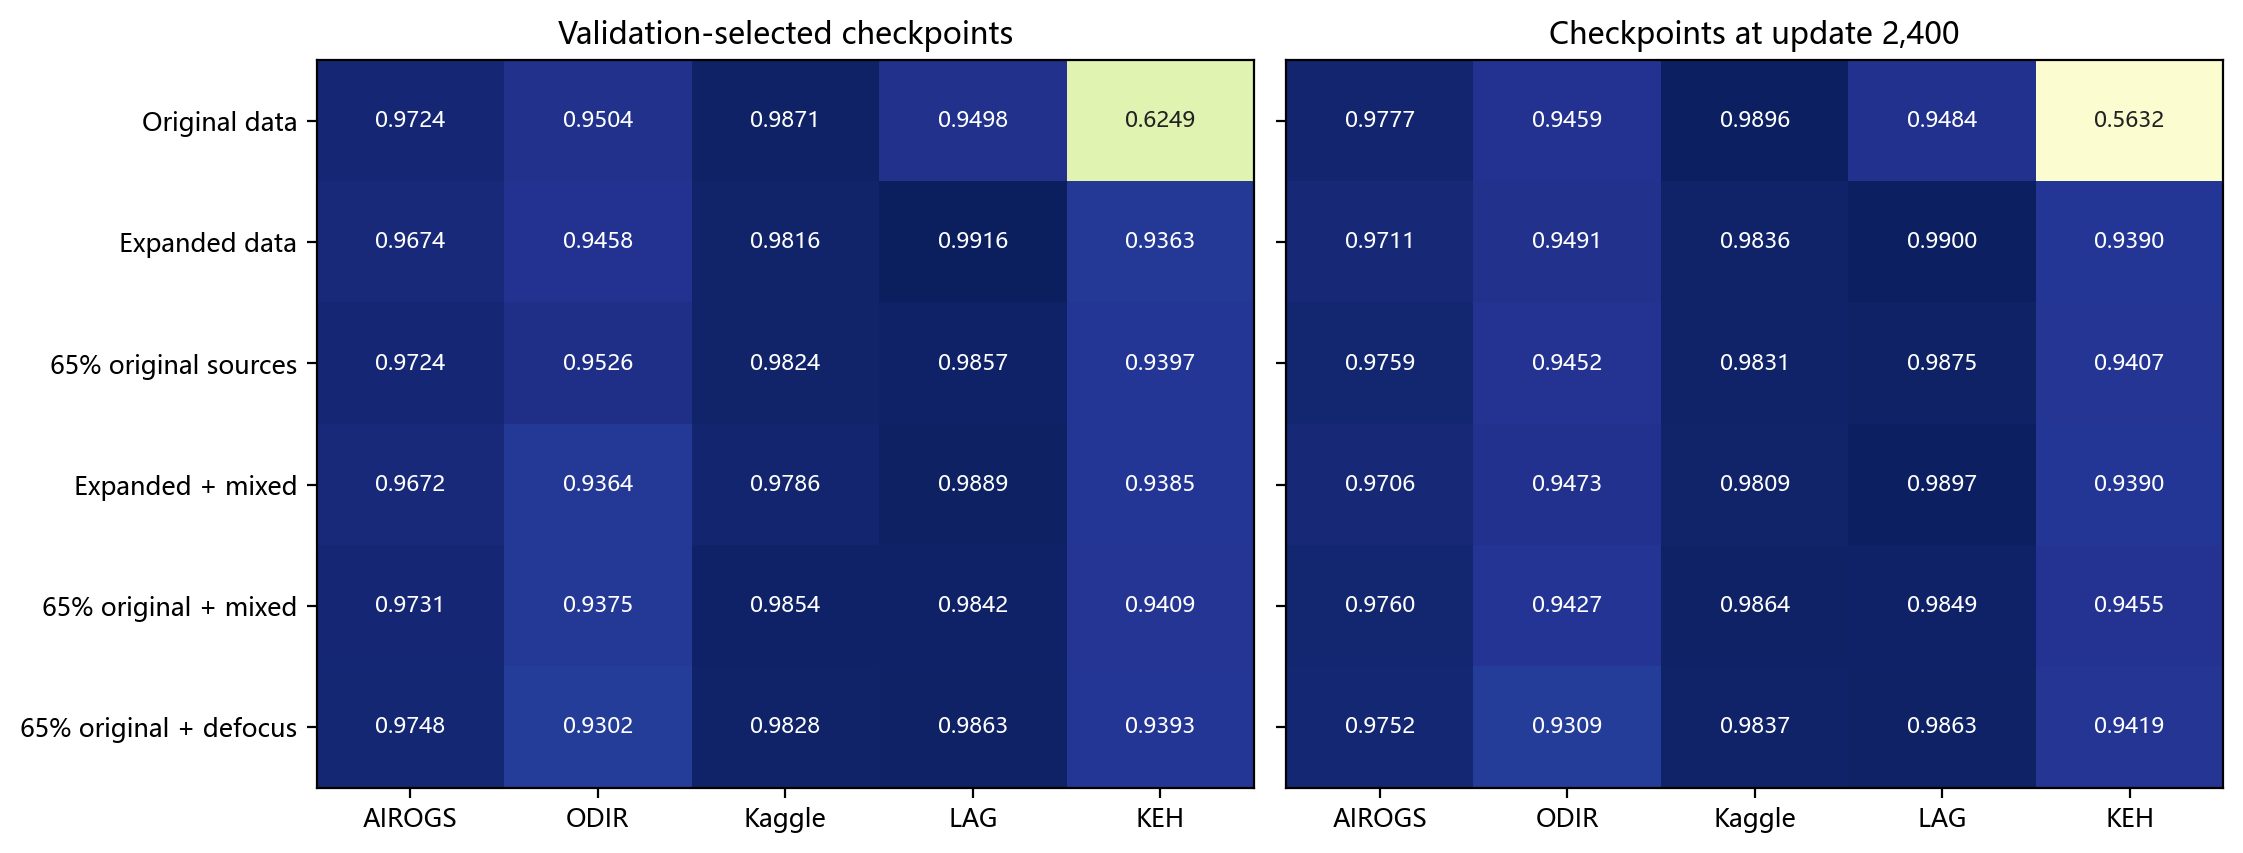
\includegraphics[keepaspectratio,alt={Source AUROC at two training stages}]{source-auroc.en.png}}
\caption{Source AUROC at two training stages}
\end{figure}

Figure 1 shows three-seed mean disease AUROC within each source. The
left panel uses validation-selected checkpoints; the right uses update
2,400 in every run. Darker cells indicate better ranking. These panels
assess performance after the specified checkpoint-selection procedure
and performance at a common update budget, respectively.

With selected checkpoints, clean expansion raises LAG from 0.9498 to
0.9916 and KEH from 0.6249 to 0.9363. The three LAG gains are +0.0472,
+0.0383, and +0.0401; KEH gains are +0.2979, +0.2769, and +0.3593.
Adding LAG and KEH as training sources provides a clear benefit from
source coverage. Pooled development AUROC increases from 0.9365 to
0.9753.

\begin{figure}[H]
\centering
\pandocbounded{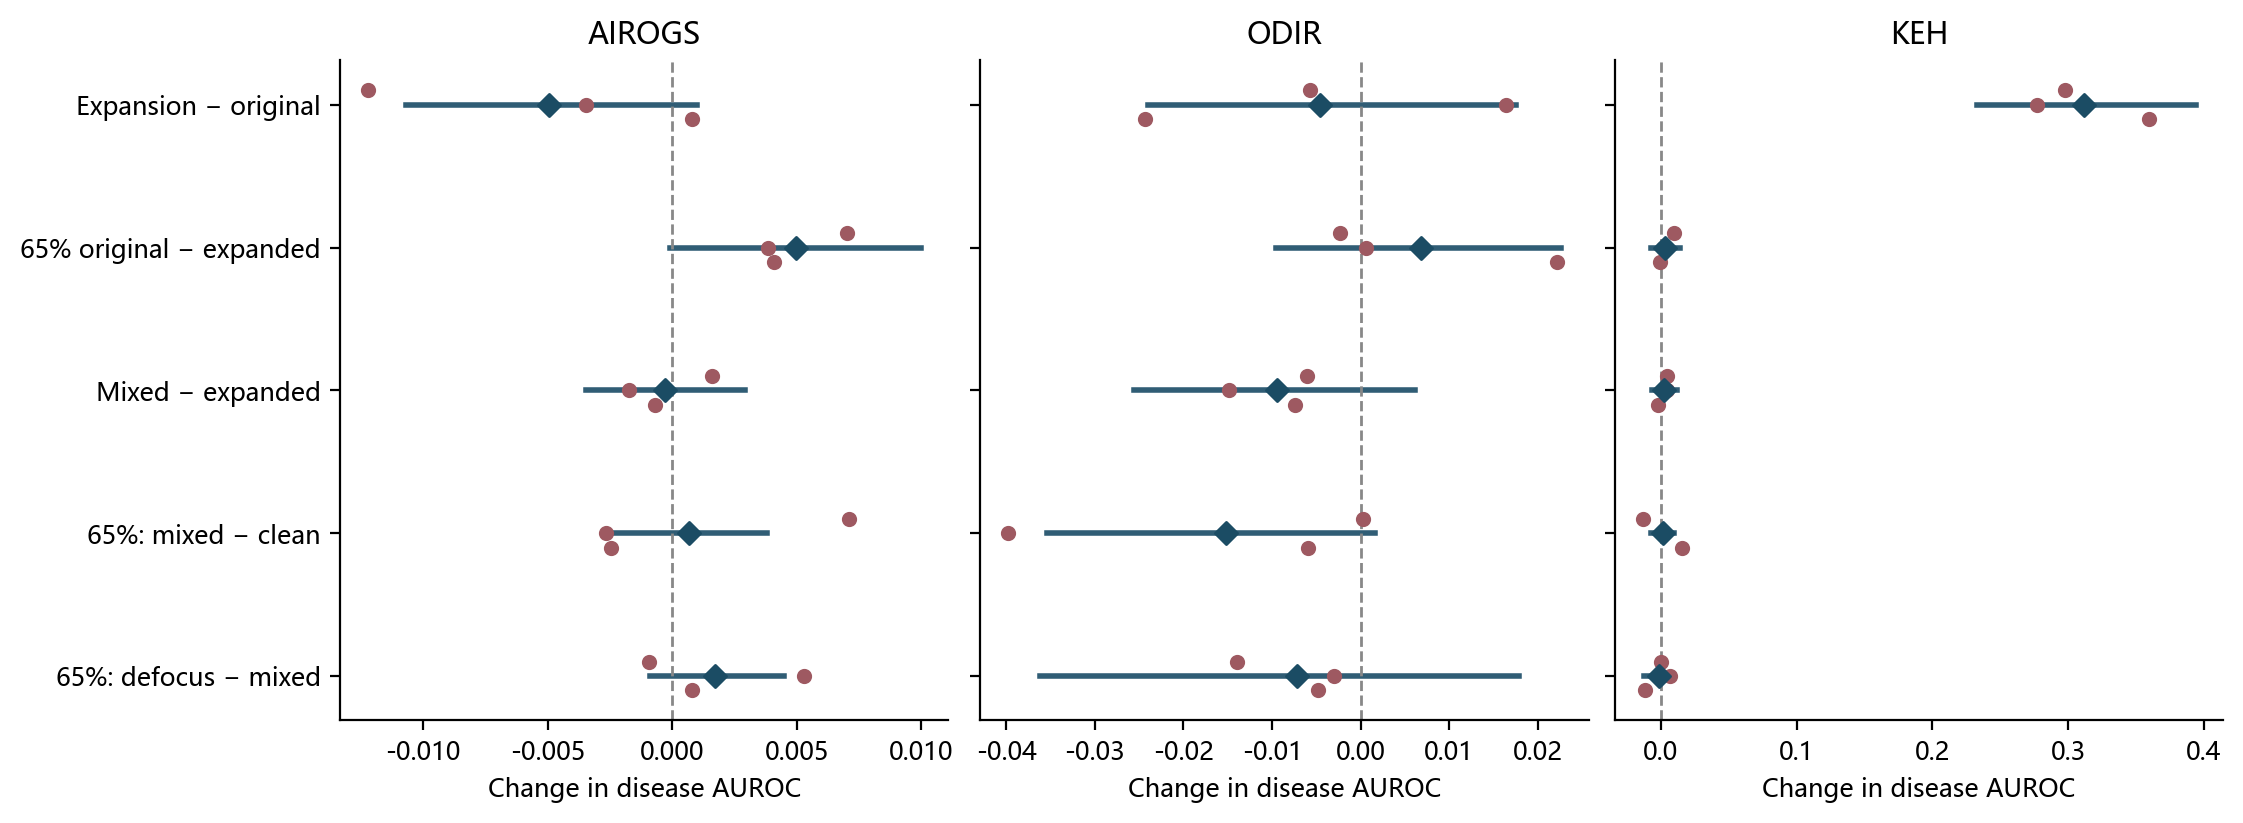
\includegraphics[keepaspectratio,alt={Paired AUROC changes in principal sources}]{paired-source-effects.en.png}}
\caption{Paired AUROC changes in principal sources}
\end{figure}

Figure 2 shows paired changes for the three common seeds as red points,
their mean as a diamond, and a 95\% interval from 2,000 resamples of the
same linked groups. Each resample uses the same cases for both
conditions and averages changes across three fixed models. Intervals
describe case sampling; individual points show training-seed variation.
The expansion interval is {[}0.0280, 0.0555{]} for LAG and {[}0.2326,
0.3940{]} for KEH.

Under current expanded sampling, original-source photographs are
presented 18,849 times on average by update 2,400, or 49.1\% of
presentations. The 65\% condition presents them 24,950 times,
approximately 32\% more often. Restoring this exposure improves selected
AIROGS AUROC in all three seeds, by +0.0070, +0.0038, and +0.0041,
averaging +0.0050. LAG declines in all three seeds, averaging −0.0059.
This is a tradeoff between training exposure to original and newly added
sources.

Selected ODIR gains from expansion are −0.0057, +0.0164, and −0.0244.
The 65\% condition changes ODIR relative to current expanded sampling by
−0.0023, +0.0006, and +0.0222. Direction varies substantially. ODIR has
28 positive photographs in 19 linked groups, with correspondingly broad
case intervals. Further sampling comparisons should report sensitivity,
false alarms, and training stage alongside AUROC.

\subsection{Selected checkpoints and end-of-budget
results}\label{selected-checkpoints-and-end-of-budget-results}

\begin{figure}[H]
\centering
\pandocbounded{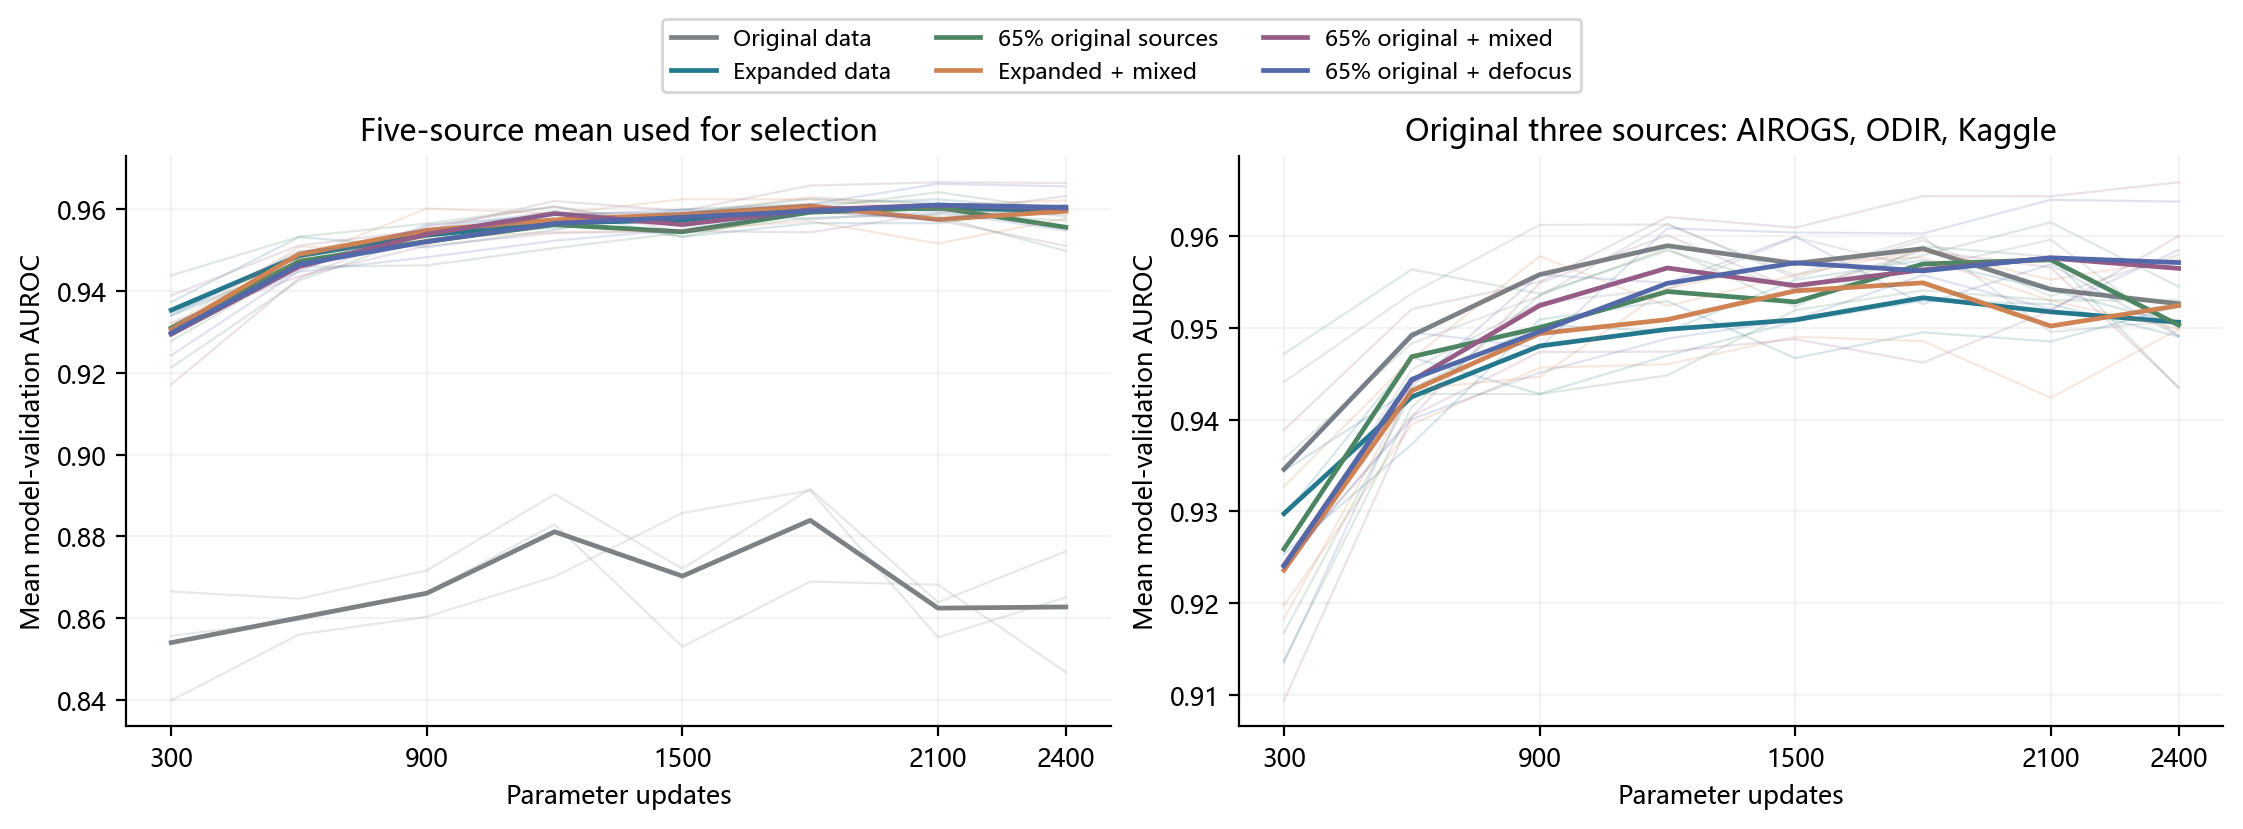
\includegraphics[keepaspectratio,alt={Complete validation curves}]{validation-curves.en.png}}
\caption{Complete validation curves}
\end{figure}

Figure 3 uses the 2,046 model-validation photographs. Thick lines are
means across three seeds; thin lines show individual seeds. The left
panel is the five-source selection mean; the right uses only the
original three sources. Expanded conditions improve five-source
performance early, with smaller later gains. KEH has a substantial
influence on the original-data control's five-source mean.

Selected updates range from 1,200 to 2,400. For 65\% original plus mixed
degradation, the selected updates are 2,400, 1,200, and 2,100;
development misses are 78, 84, and 68. At the common update-2,400
budget, misses become 78, 144, and 86, while false alarms change from
76, 109, and 101 to 76, 49, and 65. In the second seed, 60 fewer false
alarms accompany 60 additional misses, reflecting changes in scores and
threshold behavior during training.

Source means at the common update-2,400 budget follow. Individual seeds
and the information needed to calculate their standard deviations are
retained in the \href{per-seed-results.csv}{per-seed results}.

\Needspace{8\baselineskip}
\begin{longtable}[]{@{}
  >{\raggedright\arraybackslash}p{(\linewidth - 12\tabcolsep) * \real{0.14285}}
  >{\raggedright\arraybackslash}p{(\linewidth - 12\tabcolsep) * \real{0.14285}}
  >{\raggedright\arraybackslash}p{(\linewidth - 12\tabcolsep) * \real{0.14285}}
  >{\raggedright\arraybackslash}p{(\linewidth - 12\tabcolsep) * \real{0.14285}}
  >{\raggedright\arraybackslash}p{(\linewidth - 12\tabcolsep) * \real{0.14285}}
  >{\raggedright\arraybackslash}p{(\linewidth - 12\tabcolsep) * \real{0.14285}}
  >{\raggedright\arraybackslash}p{(\linewidth - 12\tabcolsep) * \real{0.14285}}@{}}
\toprule\noalign{}
\begin{minipage}[b]{\linewidth}\raggedright
Condition
\end{minipage} & \begin{minipage}[b]{\linewidth}\raggedright
AIROGS
\end{minipage} & \begin{minipage}[b]{\linewidth}\raggedright
ODIR
\end{minipage} & \begin{minipage}[b]{\linewidth}\raggedright
Kaggle
\end{minipage} & \begin{minipage}[b]{\linewidth}\raggedright
LAG
\end{minipage} & \begin{minipage}[b]{\linewidth}\raggedright
KEH
\end{minipage} & \begin{minipage}[b]{\linewidth}\raggedright
Five-source mean
\end{minipage} \\
\midrule\noalign{}
\endhead
\bottomrule\noalign{}
\endlastfoot
Original & 0.9777 & 0.9459 & 0.9896 & 0.9484 & 0.5632 & 0.8850 \\
Expanded & 0.9711 & 0.9491 & 0.9836 & 0.9900 & 0.9390 & 0.9665 \\
65\% original & 0.9759 & 0.9452 & 0.9831 & 0.9875 & 0.9407 & 0.9665 \\
Expanded + mixed & 0.9706 & 0.9473 & 0.9809 & 0.9897 & 0.9390 &
0.9655 \\
65\% + mixed & 0.9760 & 0.9427 & 0.9864 & 0.9849 & 0.9455 & 0.9671 \\
65\% + defocus & 0.9752 & 0.9309 & 0.9837 & 0.9863 & 0.9419 & 0.9636 \\
\end{longtable}

At this stage, the 65\% condition improves AIROGS by an average +0.0048
and changes ODIR by −0.0039. The ODIR direction differs from the +0.0068
mean at selected checkpoints. Subsequent comparisons will use
validation-selected checkpoints as the main result and update 2,400 as
the common-budget supplement.

\subsection{Degradation: defocus gains and actual training
exposure}\label{degradation-defocus-gains-and-actual-training-exposure}

\begin{figure}[H]
\centering
\pandocbounded{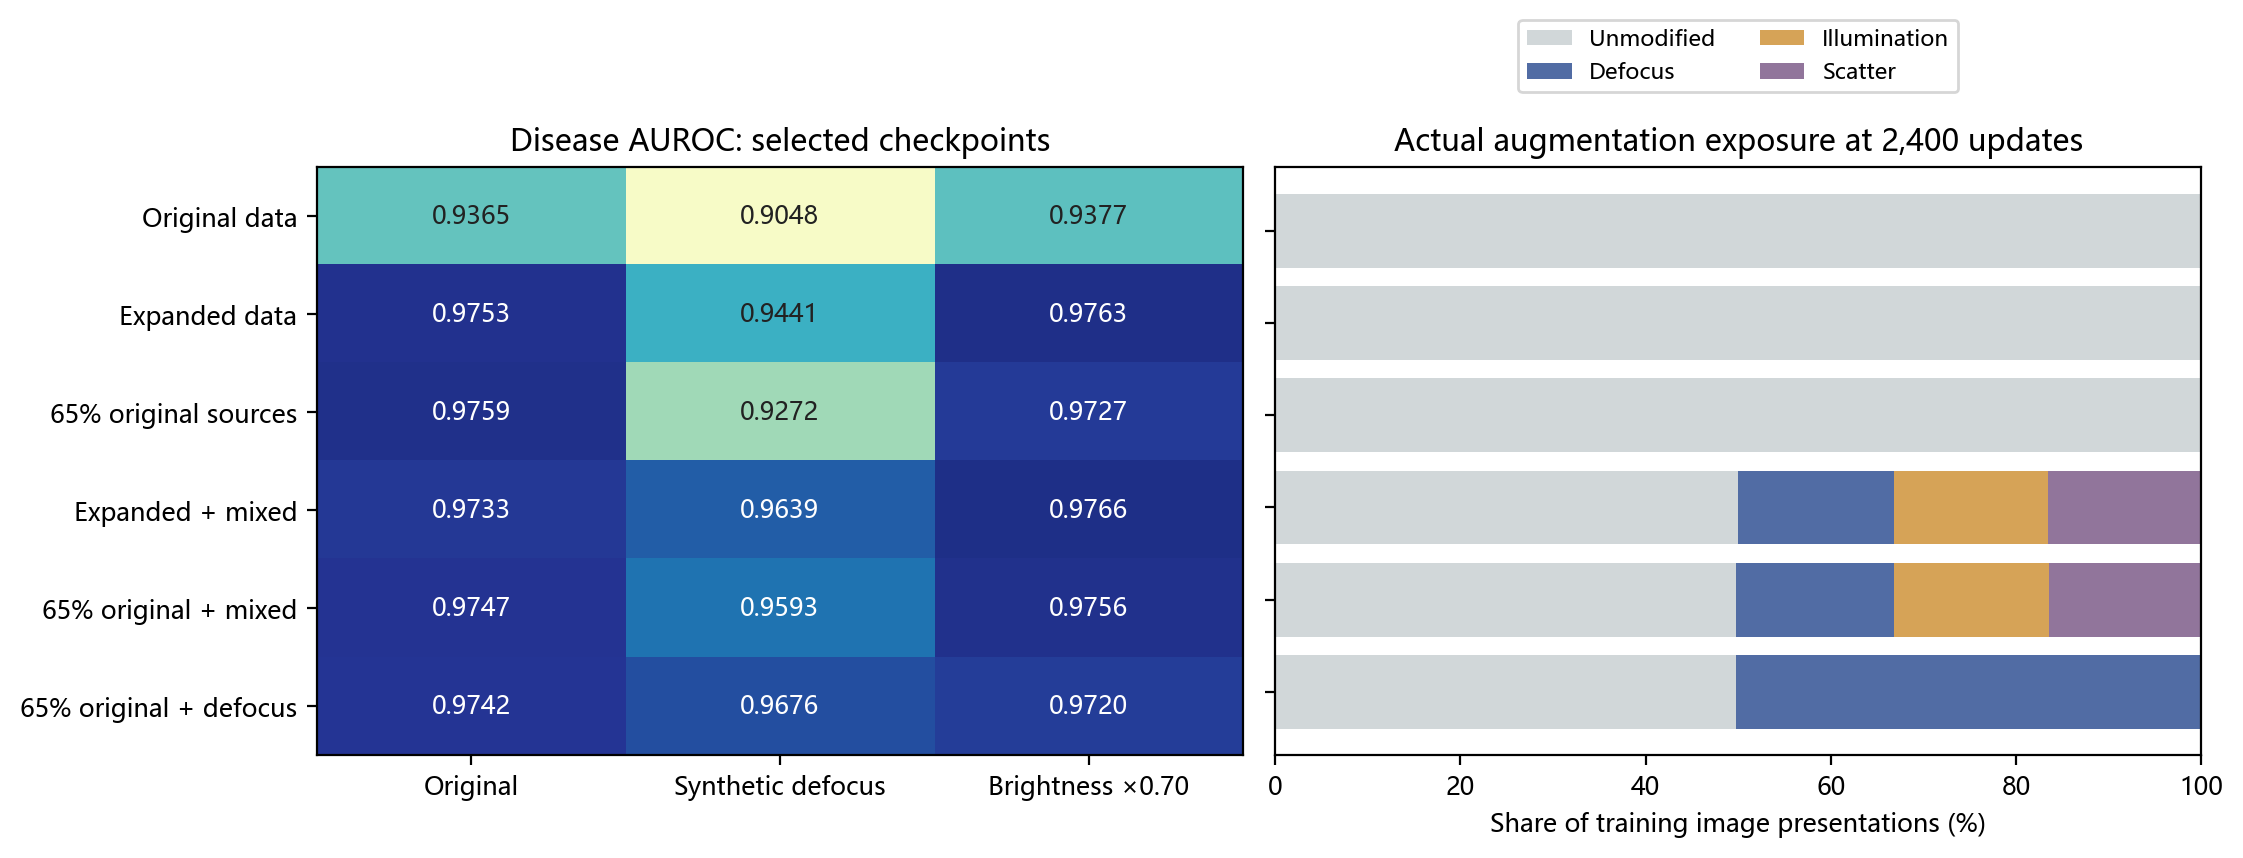
\includegraphics[keepaspectratio,alt={Synthetic stress performance and augmentation exposure}]{stress-and-training-dose.en.png}}
\caption{Synthetic stress performance and augmentation exposure}
\end{figure}

Figure 4 uses selected checkpoints. Originals contain 2,053 photographs;
each synthetic condition uses the same 384 parent images, including 146
positives and 238 negatives. Defocus applies Gaussian blur scaled to the
visible field diameter; the brightness condition multiplies brightness
by 0.70. The right panel summarizes the recorded composition of image
presentations over all 2,400 updates.

Under current expanded sampling, mixed degradation improves defocus
AUROC in all three seeds, with a mean gain of 0.0197, with case interval
{[}0.0086, 0.0316{]}. Under 65\% sampling, the mean gain is 0.0321.
Defocus-only with 65\% original sampling reaches defocus AUROC 0.9676,
compared with 0.9593 for mixed degradation, improving all three seeds.
Its five-source original-image mean decreases from 0.9642 to 0.9627,
while brightness-condition AUROC decreases from 0.9756 to 0.9720.

Exposure frequency explains part of this comparison. Defocus accounts
for approximately 17\% of all presentations under mixed degradation and
50\% under defocus-only. In the first seed these counts are 6,554 and
19,341, a 2.95-fold difference. The comparison changes both augmentation
composition and defocus frequency. A defocus-only condition with
approximately one-sixth application probability would match defocus
exposure in the mixed condition and help separate these effects.

Defocus also moves positive and negative scores toward one another. In
clean expanded models, applying synthetic defocus to the same parent
images raises negative p by 0.0590 and lowers positive p by 0.0761 on
average. With mixed degradation the changes are +0.0280 and −0.0617.
Augmentation reduces these shifts, particularly the rise in negative
scores. Detection in real poor-quality cases is assessed separately
using human quality labels.

\subsection{Misses, false alarms, and classification
thresholds}\label{misses-false-alarms-and-classification-thresholds}

\begin{figure}[H]
\centering
\pandocbounded{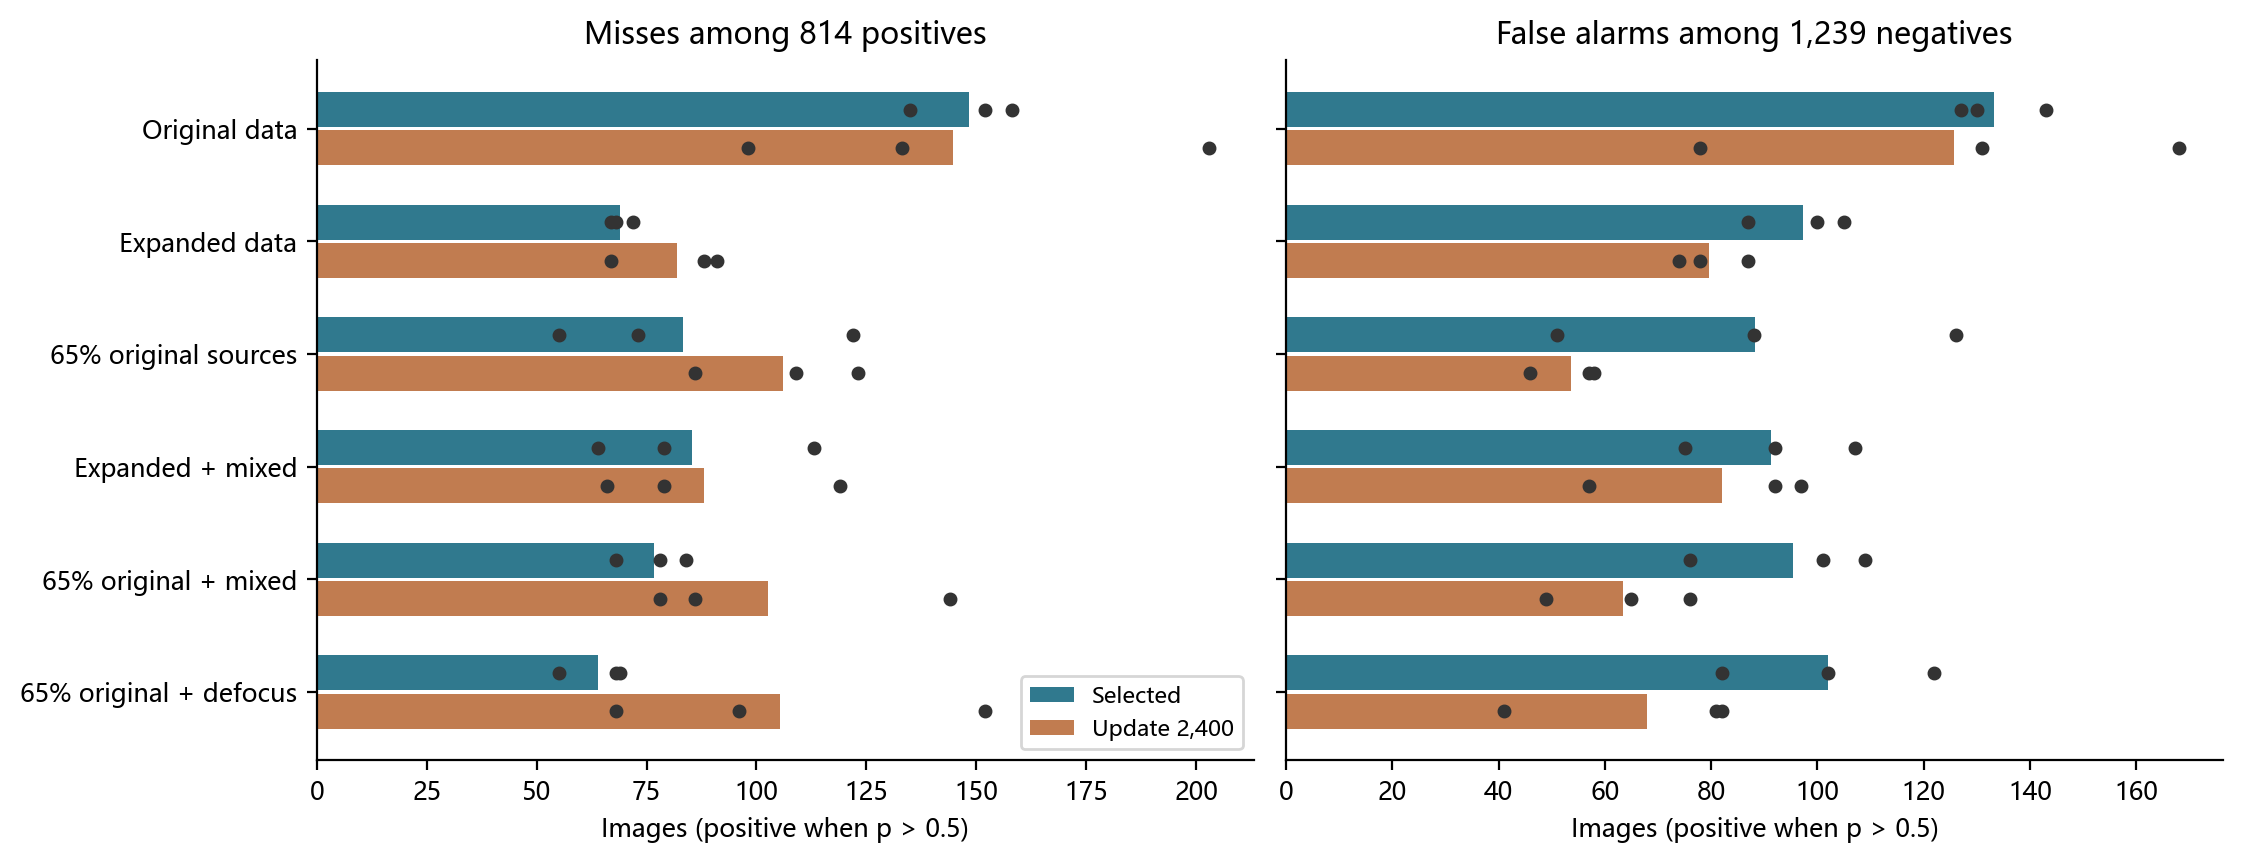
\includegraphics[keepaspectratio,alt={Misses and false alarms on original photographs}]{misses-and-false-alarms.en.png}}
\caption{Misses and false alarms on original photographs}
\end{figure}

Figure 5 uses the same 2,053 rule-development originals and
classification threshold 0.5. Bars show three-seed mean counts, with
black points for individual seeds. Blue denotes selected checkpoints and
brown update 2,400. Misses are counted among 814 positives; false alarms
among 1,239 negatives.

At selected checkpoints, clean expansion averages 69.0 misses and 97.3
false alarms; 65\% original plus mixed degradation averages 76.7 and
95.3; defocus-only averages 64.0 and 102.0. At this threshold,
defocus-only detects more positives at the cost of more false alarms. At
update 2,400, clean 65\% sampling yields 26.0 fewer false alarms and
24.0 more misses than clean expanded sampling, changing total errors by
-2.0. Total errors should be read alongside both components.

A second operating-point comparison sets each source threshold to the
95th percentile of its model-validation negative scores, then holds it
fixed for rule-development originals. Results below are means across
three seeds. The table reports the specificity actually achieved in rule
development.

\Needspace{8\baselineskip}
\begin{longtable}[]{@{}lll@{}}
\toprule\noalign{}
Condition / source & Sensitivity & Specificity \\
\midrule\noalign{}
\endhead
\bottomrule\noalign{}
\endlastfoot
Expanded / AIROGS & 83.7\% & 94.3\% \\
Expanded / ODIR & 57.1\% & 96.4\% \\
65\% + mixed / AIROGS & 84.6\% & 94.5\% \\
65\% + mixed / ODIR & 48.8\% & 97.1\% \\
65\% + defocus / AIROGS & 87.3\% & 94.1\% \\
65\% + defocus / ODIR & 46.4\% & 96.4\% \\
\end{longtable}

For ODIR, sensitivity under this procedure is 57.1\% with clean
expansion, 48.8\% with 65\% plus mixed degradation, and 46.4\% with
defocus-only. High classification AUROC can coexist with low sensitivity
at a particular threshold. Threshold selection should specify the
acceptable miss rate and show the associated false alarms and review
workload.

\subsection{Quality and errors across the complete
experiment}\label{quality-and-errors-across-the-complete-experiment}

\begin{figure}[H]
\centering
\pandocbounded{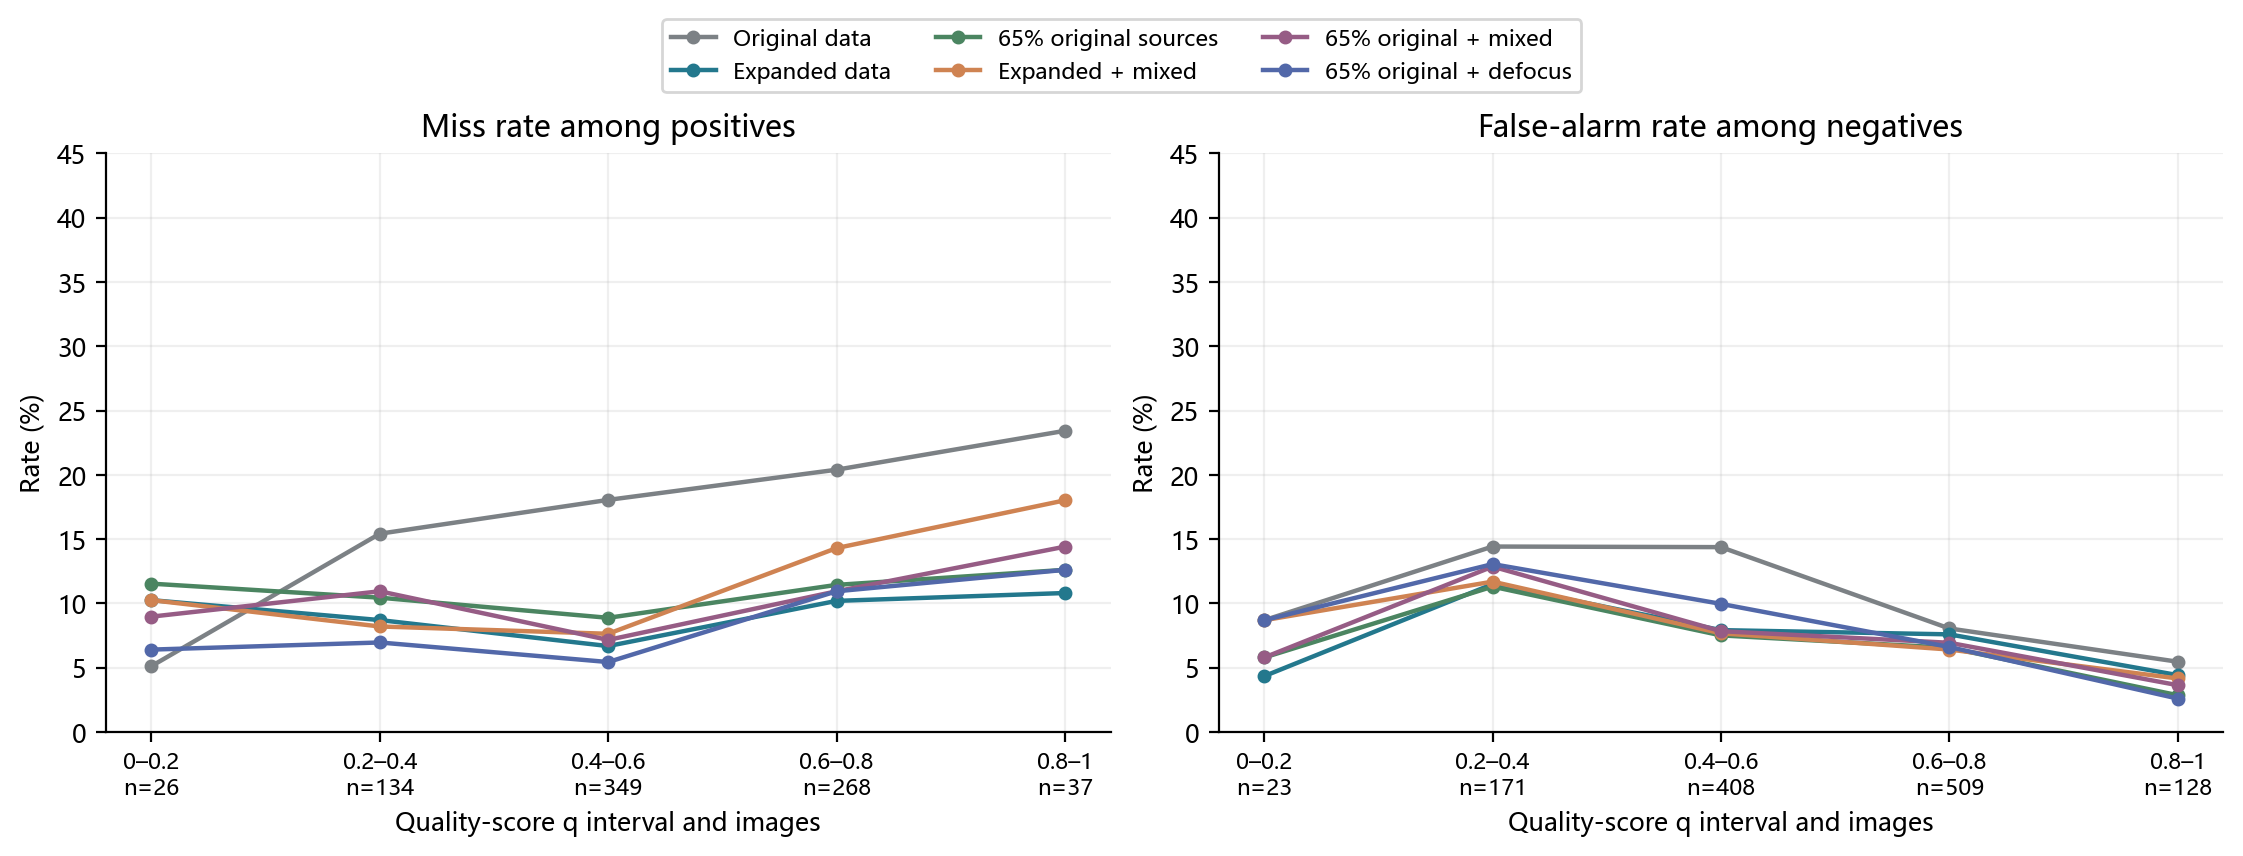
\includegraphics[keepaspectratio,alt={Miss and false-alarm rates within quality intervals}]{quality-error-rates.en.png}}
\caption{Miss and false-alarm rates within quality intervals}
\end{figure}

Figure 6 uses the original FTHNet quality score q and the 18 selected
disease models. Lines show each condition's three-seed mean error rates.
The n values below the axis are positive or negative image counts within
each interval; the same cases are evaluated in every seed. Misses and
false alarms use separate disease-class denominators.

Positive and negative composition differs across q intervals. Only 26
positives and 23 negatives have q \textless{} 0.2, while 654 positives
and 1,045 negatives have q ≥ 0.4. Many errors in moderate-to-high q
regions first reflect the large number of cases there. Positive miss
rates remain substantial in the highest-q interval: 65\% plus mixed
degradation misses 6/37, 6/37, and 4/37 across seeds. Good overall image
quality can accompany difficult disease classification.

\begin{figure}[H]
\centering
\pandocbounded{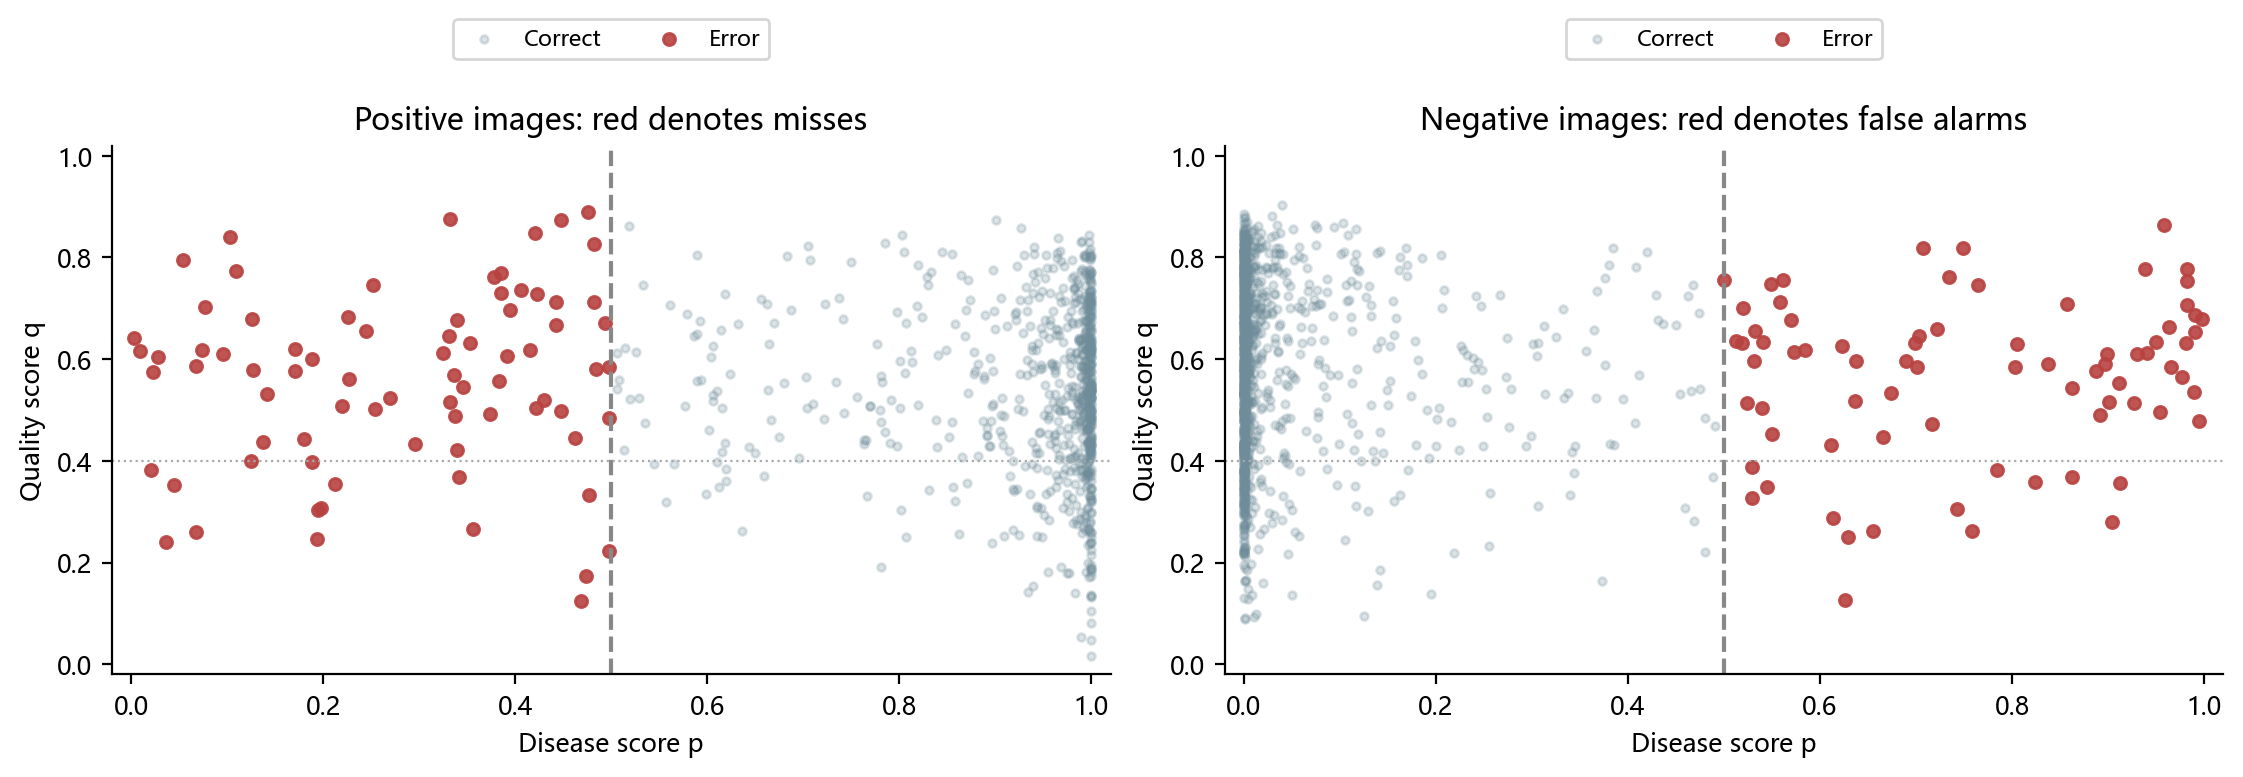
\includegraphics[keepaspectratio,alt={Joint disease-score and quality-score distribution}]{disease-quality-distribution.en.png}}
\caption{Joint disease-score and quality-score distribution}
\end{figure}

Figure 7 shows the first seed's update-2,400 rule-development results
for the condition with the highest mean validation score: 65\% original
plus mixed degradation. Blue-gray points denote correct classifications
and red points errors, with positives on the left and negatives on the
right. The vertical p=0.5 line is the classification threshold; q=0.4
marks a quality-score range for comparison. Misses and false alarms
occur at multiple quality levels, so review regions require evaluation
of p, q, and both error types.

\subsection{Additional review value of quality
scores}\label{additional-review-value-of-quality-scores}

For each fixed disease model, error ranking is fitted using five-fold
group cross-validation. All images in one linked group stay in the same
fold. The other four folds fit a model and generate predictions for the
held-out fold. Logistic regression learns how input scores relate to the
probability of error. The p-only method represents the direction of the
disease score and its distance from 0.5; adding q learns how quality and
disease scores act together. Both methods use the same folds within each
disease model; standardization is fitted within the training folds. The
comparison is repeated with the EyeQ quality model selected at epoch 17.

The AUROC below measures error ranking: the probability that a randomly
drawn error image ranks above a randomly drawn correct image, with 0.5
indicating chance. The first three metrics are three-seed means. The
final column lists the three seeds' additional errors selected after
adding FTHNet q to fitted p, when reviewing the same 411 images.

\Needspace{8\baselineskip}
\begin{longtable}[]{@{}
  >{\raggedright\arraybackslash}p{(\linewidth - 8\tabcolsep) * \real{0.2000}}
  >{\raggedright\arraybackslash}p{(\linewidth - 8\tabcolsep) * \real{0.2000}}
  >{\raggedright\arraybackslash}p{(\linewidth - 8\tabcolsep) * \real{0.2000}}
  >{\raggedright\arraybackslash}p{(\linewidth - 8\tabcolsep) * \real{0.2000}}
  >{\raggedright\arraybackslash}p{(\linewidth - 8\tabcolsep) * \real{0.2000}}@{}}
\toprule\noalign{}
\begin{minipage}[b]{\linewidth}\raggedright
Condition
\end{minipage} & \begin{minipage}[b]{\linewidth}\raggedright
Low-q AUROC
\end{minipage} & \begin{minipage}[b]{\linewidth}\raggedright
p uncertainty AUROC
\end{minipage} & \begin{minipage}[b]{\linewidth}\raggedright
Adding q: AUROC change
\end{minipage} & \begin{minipage}[b]{\linewidth}\raggedright
Adding q: extra errors
\end{minipage} \\
\midrule\noalign{}
\endhead
\bottomrule\noalign{}
\endlastfoot
Original & 0.5433 & 0.8277 & -0.0007 & -4 / -1 / +0 \\
Expanded & 0.5235 & 0.8822 & -0.0003 & +0 / +1 / +4 \\
65\% original & 0.5402 & 0.8859 & -0.0008 & -2 / -3 / +2 \\
Expanded + mixed & 0.5110 & 0.8821 & -0.0005 & +2 / -1 / +0 \\
65\% + mixed & 0.5364 & 0.8879 & -0.0008 & +2 / +1 / +0 \\
65\% + defocus & 0.5392 & 0.8749 & +0.0002 & -1 / -3 / +1 \\
\end{longtable}

\begin{figure}[H]
\centering
\pandocbounded{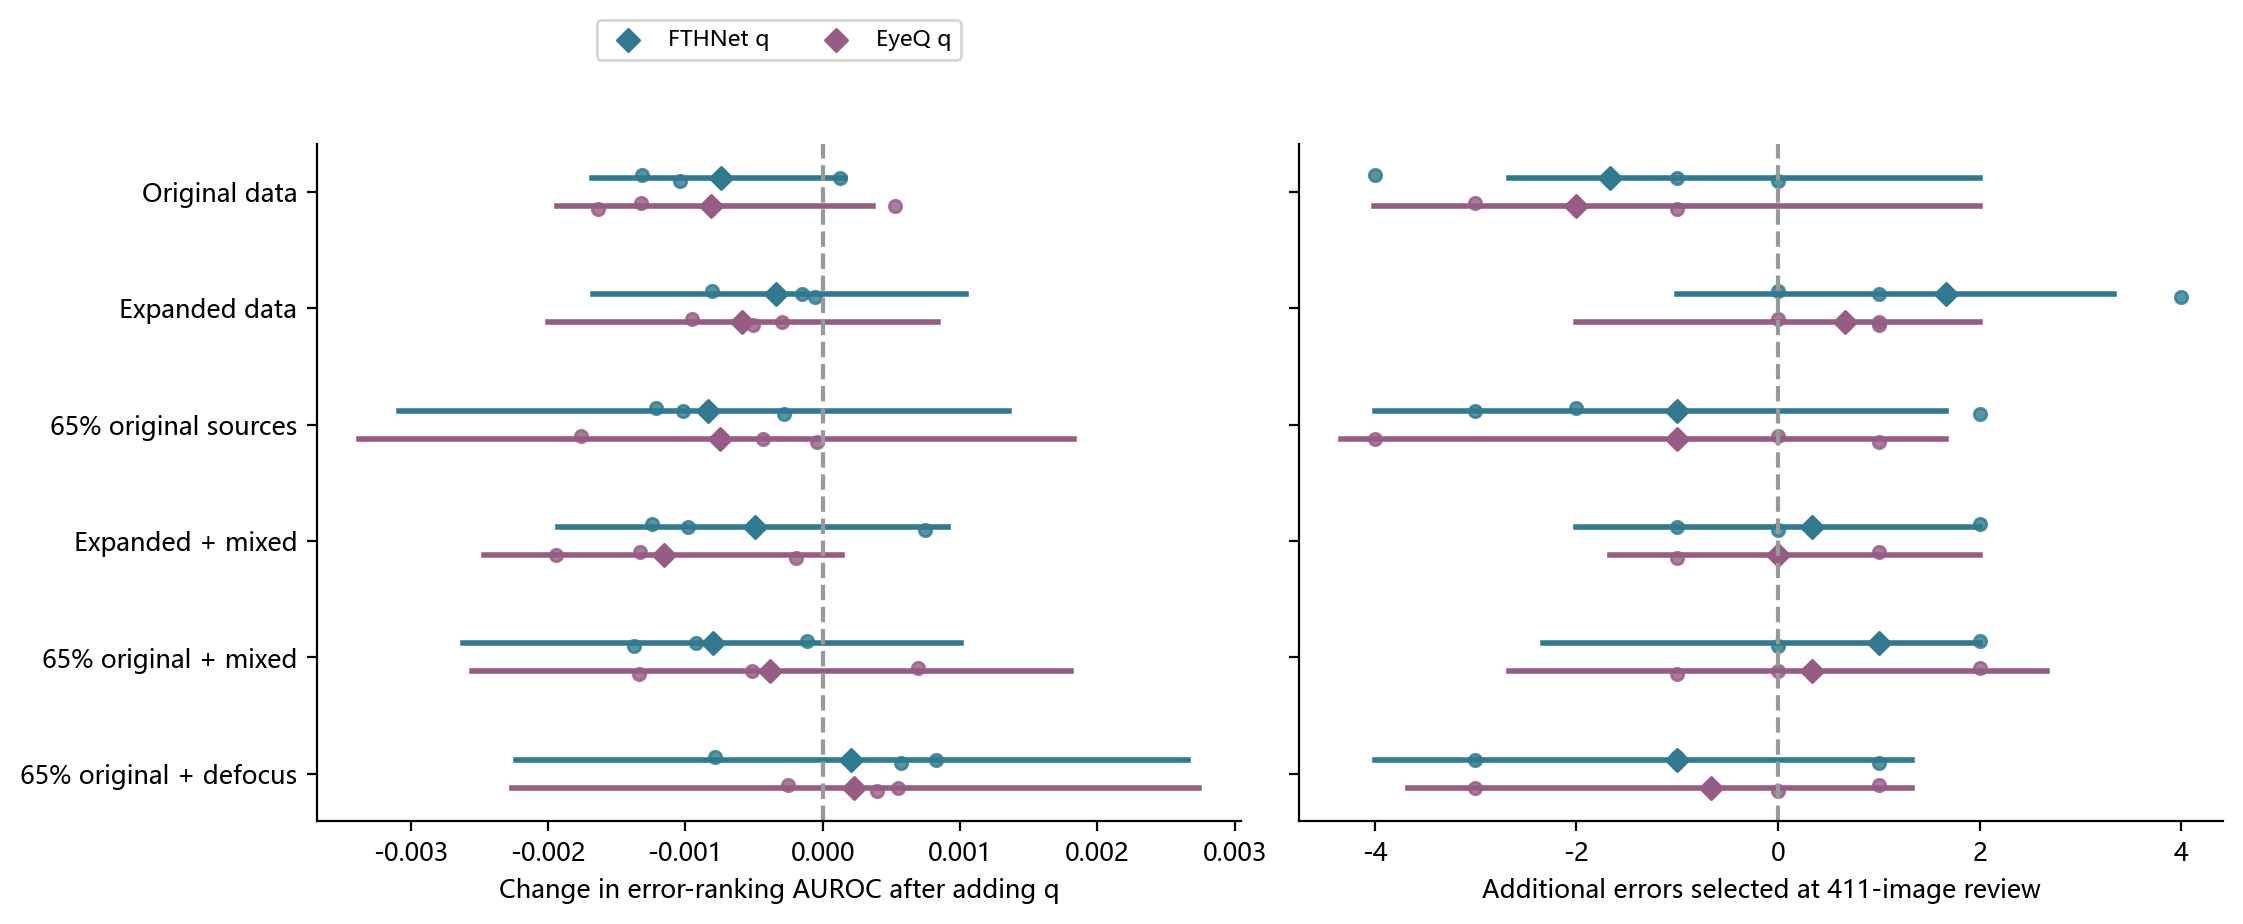
\includegraphics[keepaspectratio,alt={Additional review effects of two quality scores}]{quality-review-effects.en.png}}
\caption{Additional review effects of two quality scores}
\end{figure}

Figure 8 includes FTHNet and EyeQ comparisons for every condition.
Points denote seeds, diamonds means, and lines 95\% intervals from 2,000
paired linked-group resamples. Each resample reranks images and keeps
the reviewed count equal between methods. These intervals fix the
disease models and generated out-of-fold risks, describing variation
from case sampling.

For 65\% plus mixed degradation, adding FTHNet q changes mean error
AUROC by -0.00080, with case interval {[}-0.00262, +0.00101{]}. At 20\%
review it selects 2, 1, and 0 additional errors, averaging +1, with
interval {[}−2.33, +2.00{]}. EyeQ also provides small increments. Adding
source indicators to error models leaves the direction of q gains
varying across seeds.

\begin{figure}[H]
\centering
\pandocbounded{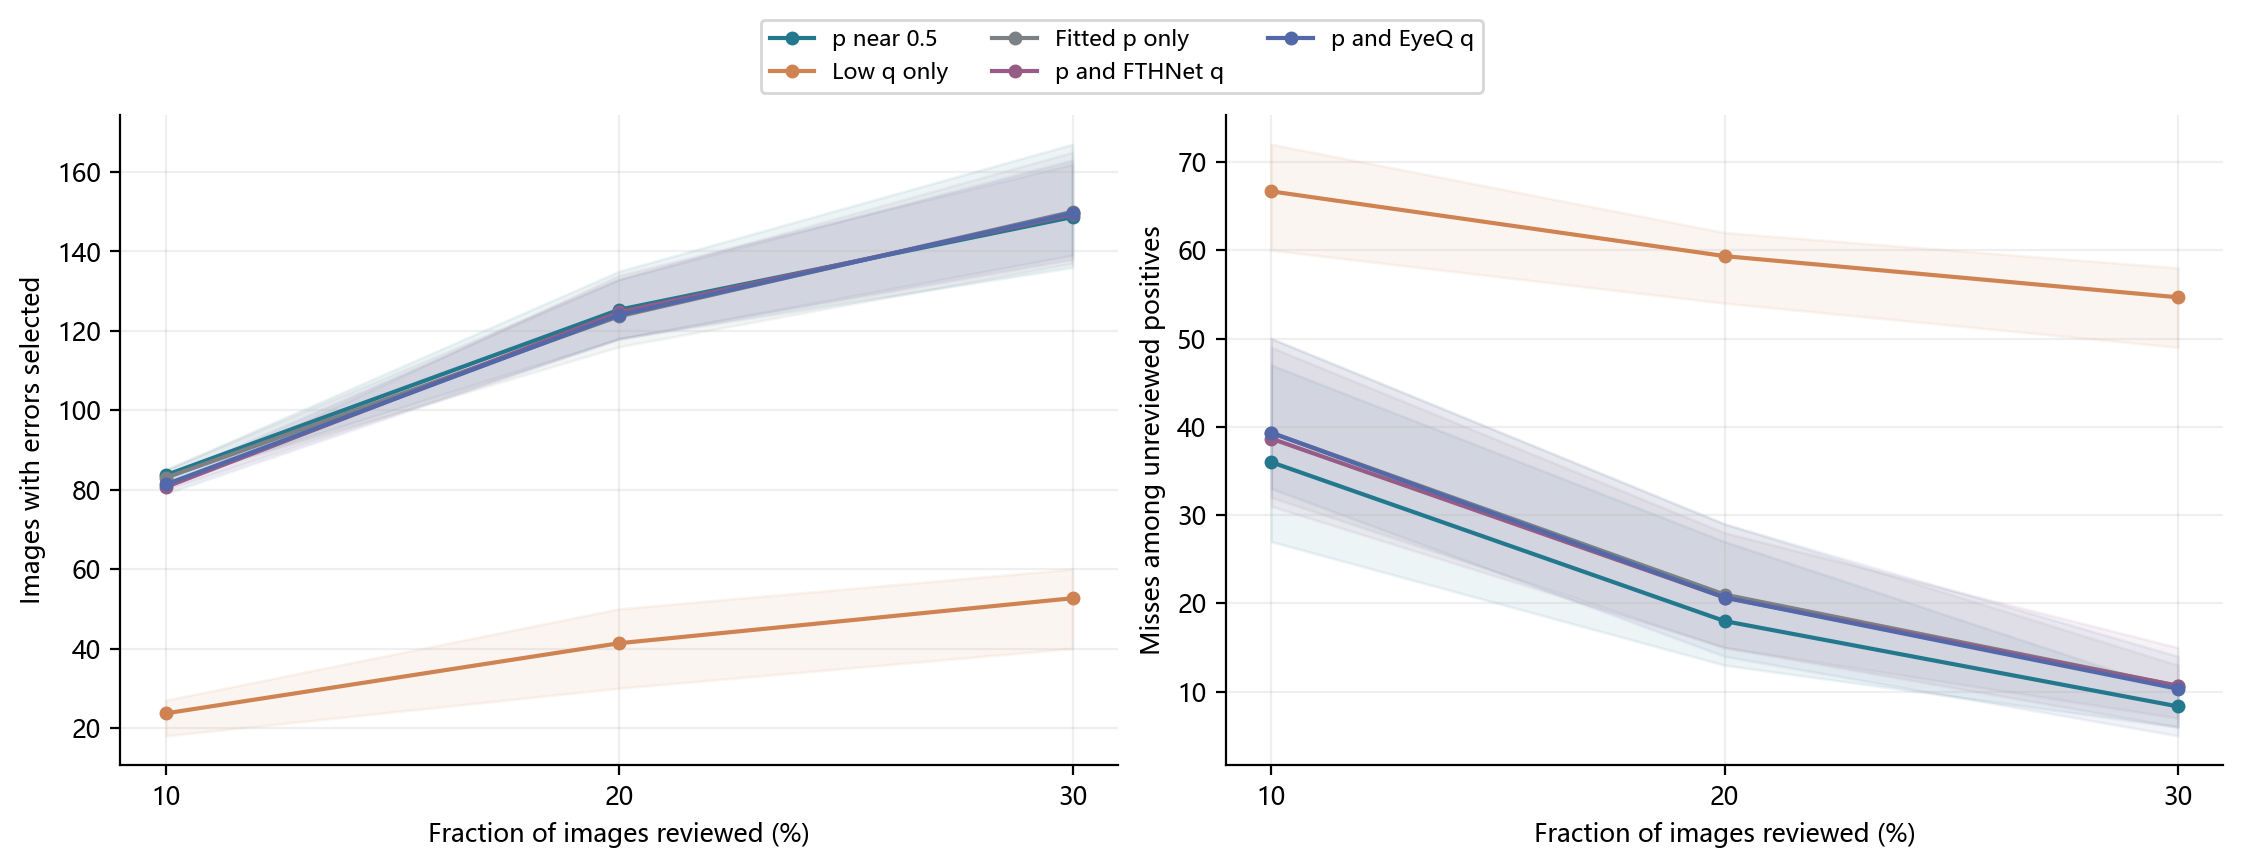
\includegraphics[keepaspectratio,alt={Review workload, selected errors, and remaining misses}]{review-workload.en.png}}
\caption{Review workload, selected errors, and remaining misses}
\end{figure}

Figure 9 uses the three selected models from 65\% plus mixed
degradation. Lines are means; shading spans the minimum and maximum
across seeds. The left panel counts errors referred for review, while
the right counts positive misses left outside review. Both use
photographs as the counting unit.

At the same 411-image workload, the following table summarizes the
methods. Averaging integer counts across three models produces
fractional values.

\Needspace{8\baselineskip}
\begin{longtable}[]{@{}
  >{\raggedright\arraybackslash}p{(\linewidth - 6\tabcolsep) * \real{0.2500}}
  >{\raggedright\arraybackslash}p{(\linewidth - 6\tabcolsep) * \real{0.2500}}
  >{\raggedright\arraybackslash}p{(\linewidth - 6\tabcolsep) * \real{0.2500}}
  >{\raggedright\arraybackslash}p{(\linewidth - 6\tabcolsep) * \real{0.2500}}@{}}
\toprule\noalign{}
\begin{minipage}[b]{\linewidth}\raggedright
Review ranking
\end{minipage} & \begin{minipage}[b]{\linewidth}\raggedright
Errors selected
\end{minipage} & \begin{minipage}[b]{\linewidth}\raggedright
Misses selected
\end{minipage} & \begin{minipage}[b]{\linewidth}\raggedright
Unreviewed misses
\end{minipage} \\
\midrule\noalign{}
\endhead
\bottomrule\noalign{}
\endlastfoot
p near 0.5 & 125.3 & 58.7 & 18.0 \\
Low q only & 41.3 & 17.3 & 59.3 \\
Fitted p only & 123.7 & 55.7 & 21.0 \\
p and FTHNet q & 124.7 & 56.0 & 20.7 \\
p and EyeQ q & 124.0 & 56.0 & 20.7 \\
\end{longtable}

Simple ranking by proximity of p to 0.5 selects 125.3 errors and 58.7
misses on average, leaving 18.0 unreviewed misses. Fitted p,q selects
124.7 errors and 56.0 misses, leaving 20.7. Photographic-quality
recognition and disease-error recognition are different tasks;
disease-score information accounts for most review gains in this round.
The proposal comparison will retain simple p ranking and fitted p within
the same classifier as controls, judging q by additional errors or
misses captured at a specified review workload.

\subsection{How real poor-quality samples affect
interpretation}\label{how-real-poor-quality-samples-affect-interpretation}

\begin{figure}[H]
\centering
\pandocbounded{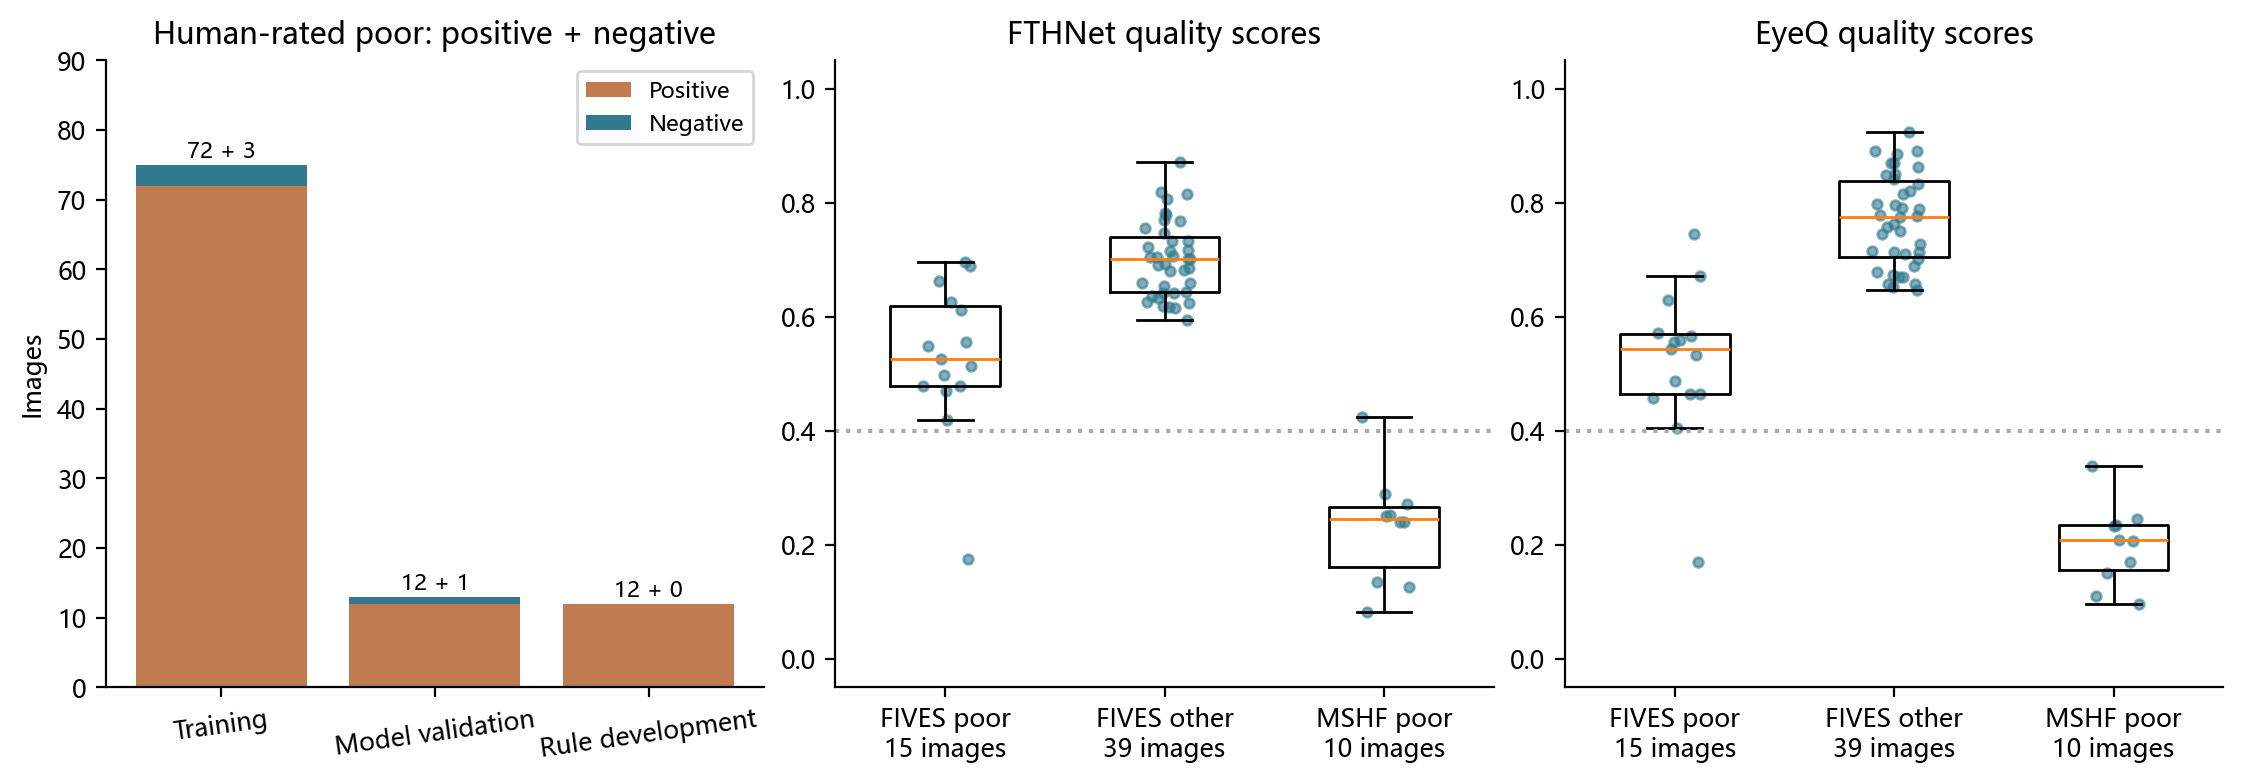
\includegraphics[keepaspectratio,alt={Human quality composition and two quality-score models}]{real-quality-composition.en.png}}
\caption{Human quality composition and two quality-score models}
\end{figure}

Figure 10 summarizes the disease-label composition and allocation of
human-rated poor-quality FIVES and MSHF photographs on the left; labels
are positive + negative. The score panels use 54 FIVES and 10 MSHF
originals from model validation and rule development. Points are
photographs, boxes the interquartile range, and lines medians. FIVES
defines poor quality as at least one poor dimension; MSHF uses its
official overall quality grade.

Training contains 72 human-rated poor-quality positives and three
negatives. Rule development contains 12 positives and no negatives;
model validation contains one poor-quality negative. All 15 expanded
models detect these 12 positives, while original-data controls miss 5,
5, and 4. Clean expansion also achieves 12/12, showing that detection
improvement in this group already accompanies data expansion. Zero
misses in 12 independent cases gives a one-sided 95\% upper miss-rate
bound of 22.1\%. Poor-quality false alarms require independent negative
cases for estimation.

The shortage has two components: few real poor-quality cases overall,
and strong association of poor quality with disease label and source.
Resampling increases presentations of the same cases; synthetic
degradation adds transformations of existing cases. Real poor-quality
negative acquisition can improve both training composition and
false-alarm evaluation. Acquisition should prioritize independent cases
with the same source and collection conditions, an explicit negative
glaucoma diagnosis, and human quality labels. Under zero errors, at
least 59 independent positives and separately 59 negatives would put
each one-sided 95\% error-rate bound below 5\%; these are minimum
planning references.

Human grades and continuous quality scores also require source-specific
interpretation. The 15 human-rated poor FIVES development images have
median q 0.5261, with only one below 0.4. The ten poor MSHF images have
median 0.2453, with nine below 0.4. Within FIVES, FTHNet distinguishes
poor human quality with AUROC 0.9026; EyeQ reaches 0.9641. Both models
distinguish photographic quality; the weak result here is their
additional ranking information for disease errors. Further human review
should record overall image quality and the visibility of diagnostic
optic-disc information.

\subsection{Next steps}\label{next-steps}

Under the existing five-source validation criterion, 65\% original plus
mixed degradation is the candidate for subsequent work, with three-seed
mean 0.9634. Its highest validation score is seed 20261117 at update
2,100, with mean 0.9665. Clean expansion remains the principal control
for data expansion and quality review. The candidate condition's mean
pooled development AUROC is 0.9747; at classification threshold 0.5 it
averages 76.7 misses and 95.3 false alarms.

The priorities are to acquire real poor-quality negatives and
independent positives with source-specific quality evaluation; select
classification thresholds and compare residual misses and false alarms
at equal review workloads while retaining disease-score controls; and
match defocus presentations to separate defocus frequency from the other
mixed transformations. Once models, thresholds, and review regions are
specified, final testing will follow the frozen allocations.

Evidence is available in the \href{completed-analysis.json}{analysis
JSON} and \href{per-seed-results.csv}{per-seed CSV}; methods are
implemented in the
\href{../../../../tools/analyze_completed_followup_20261115.py}{analysis
program} and
\href{../../../../tools/report_completed_followup_20261115.py}{report
generator}. The
\href{../../../../runs/followup_20261115/pipeline/status.json}{execution
status} records 18 completed runs. The
\href{../quality-and-training.en.md}{earlier quality analysis} preserves
the training-launch snapshot. Chinese and English Markdown, PDF, LaTeX,
and ten sets of bilingual figures share this directory.

\end{document}
